\documentclass[letterpaper, 12pt]{article}
\textwidth=6.5in
\textheight=9.5in
\topmargin=-0.75in
\oddsidemargin=0.0in
\evensidemargin=0.0in

\usepackage{graphicx}
\usepackage{enumitem}
\usepackage{amssymb, amsmath}
\usepackage{xcolor}
\usepackage{listings}

\usepackage{times}
\usepackage{natbib}
\usepackage{etoolbox}
\usepackage{astjnlabbrev-jh}
\usepackage{bibentry}
\usepackage{ifthen}
\usepackage{epsfig}

\usepackage{commath}
\usepackage{rotating}

\usepackage{dirtree}
\usepackage{changepage}
\usepackage{alltt}

%\usepackage[T1]{fontenc}
%\usepackage[scaled]{beramono}
%\usepackage[utf8]{inputenc}
%\renewcommand*\familydefault{\ttdefault}

% \lstset{
% language=Python,
% showstringspaces=false,
% formfeed=\newpage,
% tabsize=4,
% commentstyle=\itshape,
% basicstyle=\ttfamily,
% morekeywords={models, lambda, forms}
% }
 
% \newcommand{\code}[2]{
% \hrulefill
% \subsection*{#1}
% \lstinputlisting{#2}
% \vspace{2em}
% }

% Default fixed font does not support bold face
\DeclareFixedFont{\ttb}{T1}{txtt}{bx}{n}{10} % for bold
\DeclareFixedFont{\ttm}{T1}{txtt}{m}{n}{10}  % for normal
% twelve-sized ttm:
\DeclareFixedFont{\tttb}{T1}{txtt}{bx}{n}{12}  % for bold
\DeclareFixedFont{\tttm}{T1}{txtt}{m} {n}{12}  % for normal

\DeclareFixedFont{\ttnm}{T1}{txtt}{m}{n}{9.8}  % for normal

% Custom colors
\usepackage{color}
\definecolor{deepblue}  {rgb}{0.0, 0.0, 0.5}
\definecolor{deepred}   {rgb}{0.8, 0.0, 0.0}
\definecolor{deepgreen} {rgb}{0.0, 0.5, 0.0}
\definecolor{commentc}  {rgb}{0.5, 0.5, 0.5}
\definecolor{DodgerBlue}{rgb}{0.1, 0.6, 1.0}

% Python style for highlighting
\newcommand\pythonstyle{\lstset{
language=Python,
basicstyle = \ttm,
morekeywords = {self, as, assert, with, yield}, % Add keywords here
keywordstyle  = \ttb\color{blue},      %
emph        = {MyClass, __init__},     % Custom highlighting
emphstyle   = \ttb\color{DodgerBlue},  % Custom  highlighting style
stringstyle = \color{deepred},         % Strings highlighting style
commentstyle=\color{commentc},         % Comment highlighting style
frame       = tb,                      % Any extra options here
showstringspaces = false
}}

% Python environment:
\lstnewenvironment{python}[1][]{\pythonstyle\lstset{#1}}{}
% Python for external files:
\newcommand\pythonexternal[2][]{{\pythonstyle\lstinputlisting[#1]{#2}}}
% Python for inline:
\newcommand\pythoninline[1]{{\pythonstyle\lstinline!#1!}}

% Python style for highlighting
\newcommand\plainstyle{\lstset{
language=Python,
basicstyle = \ttnm,
keywordstyle  = \ttnm,      %
emph        = {MyClass, __init__},     % Custom highlighting
emphstyle   = \ttnm\color{black},    % Custom  highlighting style
stringstyle = \color{black},         % Strings highlighting style
commentstyle=\color{black},         % Comment highlighting style
frame       = tb,                      % Any extra options here
showstringspaces = false
}}

% Plain environment:
\lstnewenvironment{plain}[1][]{\plainstyle\lstset{#1}}{\vspace{10pt}}
\newcommand\plaininline[1]{{\plainstyle\lstinline!#1!}}

% To use boldface verbatim:
%\lstset{basicstyle=\ttfamily,
%        escapeinside={||},
%        mathescape=true}

\lstset{
    language={[LaTeX]TeX},
    basicstyle=\tt\color{red},
    escapeinside={||},
}

\bibliographystyle{apj_hyperref}
\usepackage[%pdftex,      %%% hyper-references for pdflatex
bookmarks=true,           %%% generate bookmarks ...
bookmarksnumbered=true,   %%% ... with numbers
colorlinks=true,          % links are colored
citecolor=blue,           % green   % color of cite links
linkcolor=blue,           %cyan,         % color of hyperref links
menucolor=blue,           % color of Acrobat Reader menu buttons
urlcolor=blue,            % color of page of \url{...}
breaklinks=true,
linkbordercolor={0 0 1},  %%% blue frames around links
pdfborder={0 0 1},
frenchlinks=true]{hyperref}
%\usepackage{breakurl}

\newcommand{\eprint}[1]{\href{http://arxiv.org/abs/#1}{#1}}
\newcommand{\ISBN}[1]{\href{http://cosmologist.info/ISBN/#1}{ISBN: #1}}
\providecommand{\adsurl}[1]{\href{#1}{ADS}}

% hyper ref only the year in citations:
\makeatletter
% Patch case where name and year are separated by aysep:
\patchcmd{\NAT@citex}
  {\@citea\NAT@hyper@{%
     \NAT@nmfmt{\NAT@nm}%
     \hyper@natlinkbreak{\NAT@aysep\NAT@spacechar}{\@citeb\@extra@b@citeb}%
     \NAT@date}}
  {\@citea\NAT@nmfmt{\NAT@nm}%
   \NAT@aysep\NAT@spacechar\NAT@hyper@{\NAT@date}}{}{}
% Patch case where name and year are separated by opening bracket:
\patchcmd{\NAT@citex}
  {\@citea\NAT@hyper@{%
     \NAT@nmfmt{\NAT@nm}%
     \hyper@natlinkbreak{\NAT@spacechar\NAT@@open\if*#1*\else#1\NAT@spacechar\fi}%
       {\@citeb\@extra@b@citeb}%
     \NAT@date}}
  {\@citea\NAT@nmfmt{\NAT@nm}%
   \NAT@spacechar\NAT@@open\if*#1*\else#1\NAT@spacechar\fi\NAT@hyper@{\NAT@date}}
  {}{}
\makeatother


%\def\bibAnnoteFile#1{}
%\bibpunct[, ]{(}{)}{,}{a}{}{,}

% Packed reference list:
\setlength\bibsep{0pt}

% \pagestyle{myheadings}
% \markright{MC\sp{3}}
% \pagenumbering{arabic}


% :::::::::::::::::::::::
\newcommand\degree{\degr}
\newcommand\degrees{\degree}
\newcommand\vs{\emph{vs.}}

% unslanted mu, for ``micro'' abbrev.
\DeclareSymbolFont{UPM}{U}{eur}{m}{n}
\DeclareMathSymbol{\umu}{0}{UPM}{"16}
\let\oldumu=\umu
\renewcommand\umu{\ifmmode\oldumu\else\math{\oldumu}\fi}
\newcommand\micro{\umu}
\newcommand\micron{\micro m}
\newcommand\microns{\micron}

\let\oldsim=\sim
\renewcommand\sim{\ifmmode\oldsim\else\math{\oldsim}\fi}
\let\oldpm=\pm
\renewcommand\pm{\ifmmode\oldpm\else\math{\oldpm}\fi}
\newcommand\by{\ifmmode\times\else\math{\times}\fi}
\newcommand\ttt[1]{10\sp{#1}}
\newcommand\tttt[1]{\by\ttt{#1}}
\newcommand\tablebox[1]{\begin{tabular}[t]{@{}l@{}}#1\end{tabular}}
\newbox{\wdbox}
\renewcommand\c{\setbox\wdbox=\hbox{,}\hspace{\wd\wdbox}}
\renewcommand\i{\setbox\wdbox=\hbox{i}\hspace{\wd\wdbox}}
\newcommand\n{\hspace{0.5em}}
\newcommand\marnote[1]{\marginpar{\raggedright\tiny\ttfamily\baselineskip=9pt #1}}
\newcommand\herenote[1]{{\bfseries #1}\typeout{======================> note on page \arabic{page} <====================}}
\newcommand\fillin{\herenote{fill in}}
\newcommand\fillref{\herenote{ref}}
\newcommand\findme[1]{\herenote{(FINDME: #1)}}

\newcount\timect
\newcount\hourct
\newcount\minct
\newcommand\now{\timect=\time \divide\timect by 60
         \hourct=\timect \multiply\hourct by 60
         \minct=\time \advance\minct by -\hourct
         \number\timect:\ifnum \minct < 10 0\fi\number\minct}

\newcommand\citeauthyear[1]{\citeauthor{#1} \citeyear{#1}}

\newcommand\mc{\multicolumn}
\newcommand\mctc{\multicolumn{2}{c}}


% {\tttm -h, --help} \\
% Print the list of arguments. \newline

% \newenvironment{myindentpar}[1]%
%   {\begin{list}{}%
%          {\setlength{\leftmargin}{3cm}}%
%      \item[]%
%   }
% {\end{list}}

\newenvironment{packed_enum}{
\begin{enumerate}[leftmargin=3cm]
   \setlength{\itemsep}{1pt}
   \setlength{\parskip}{5pt}
   \setlength{\parsep}{0pt}
}{\end{enumerate}}

\newcommand{\argument}[2]{{\noindent\tttm #1}%
\begin{adjustwidth}{2.5em}{0pt}%
#2 \vspace{0.3cm}%
\end{adjustwidth}%
}

%\newcommand{\ttmb}[1]{\tttm\color{#1}}
\newcommand{\routine}[2]{{\noindent\tttm\color{blue} #1:}%
\begin{adjustwidth}{2.0em}{0pt}%
#2 \vspace{0.15cm}%
\end{adjustwidth}%
}

% \newcommand{\routine}[2]{{\noindent\tttm\color{blue} #1}%
% \begin{adjustwidth}{0.0em}{0pt}%
%  #2 \vspace{0.15cm}%
% \end{adjustwidth}%
% }

% :::::::::::::::::: jhmacs2.tex :::::::::::::::::::::::::::::::::::::
\typeout{Joe Harrington's personal setup, Wed Jun 17 10:53:17 EDT 1998}
% Tue Mar 29 22:23:03 EST 1994

% :::::: pato.tex ::::::
% Joetex character unreservations.
% This file frees most of TeX's reserved characters, and provides
% several alternatives for their functions.


% utility
\catcode`@=11

% comments are first....
\newcommand\comment[1]{}

\newcommand\commenton{\catcode`\%=14}
\newcommand\commentoff{\catcode`\%=12}

% Not-a-comment:
\newcommand\nocomment[1]{#1}

\renewcommand\math[1]{$#1$}
\newcommand\mathshifton{\catcode`\$=3}
\newcommand\mathshiftoff{\catcode`\$=12}

\comment{alignment tab}
\let\atab=&
\newcommand\atabon{\catcode`\&=4}
\newcommand\ataboff{\catcode`\&=12}

\let\oldmsp=\sp
\let\oldmsb=\sb
\def\sp#1{\ifmmode
           \oldmsp{#1}%
         \else\strut\raise.85ex\hbox{\scriptsize #1}\fi}
\def\sb#1{\ifmmode
           \oldmsb{#1}%
         \else\strut\raise-.54ex\hbox{\scriptsize #1}\fi}
\newbox\@sp
\newbox\@sb
\def\sbp#1#2{\ifmmode%
           \oldmsb{#1}\oldmsp{#2}%
         \else
           \setbox\@sb=\hbox{\sb{#1}}%
           \setbox\@sp=\hbox{\sp{#2}}%
           \rlap{\copy\@sb}\copy\@sp
           \ifdim \wd\@sb >\wd\@sp
             \hskip -\wd\@sp \hskip \wd\@sb
           \fi
        \fi}
\def\msp#1{\ifmmode
           \oldmsp{#1}
         \else \math{\oldmsp{#1}}\fi}
\def\msb#1{\ifmmode
           \oldmsb{#1}
         \else \math{\oldmsb{#1}}\fi}
\def\supon{\catcode`\^=7}
\def\supoff{\catcode`\^=12}
\def\subon{\catcode`\_=8}
\def\suboff{\catcode`\_=12}
\def\supsubon{\supon \subon}
\def\supsuboff{\supoff \suboff}


\newcommand\actcharon{\catcode`\~=13}
\newcommand\actcharoff{\catcode`\~=12}

\newcommand\paramon{\catcode`\#=6}
\newcommand\paramoff{\catcode`\#=12}

\comment{And now to turn us totally on and off...}

\newcommand\reservedcharson{ \commenton  \mathshifton  \atabon  \supsubon
                             \actcharon  \paramon}

\newcommand\reservedcharsoff{\commentoff \mathshiftoff \ataboff \supsuboff
                             \actcharoff \paramoff}

\newcommand\nojoe[1]{\reservedcharson #1 \reservedcharsoff}

\catcode`@=12
\reservedcharsoff

\reservedcharson
\newcommand\jhauth[1]{{#1}}
\newcommand\jhstud[1]{{#1}}

\comment{Must have ONLY ONE of these... trust these macros, they work
\newcommand\jhauth[1]{{\bfseries #1}}
\newcommand\jhstud[1]{{\em #1}}
}

\reservedcharsoff
\reservedcharson


% ::::::::::::::::::::::::::::::::::::::::::::::::::::

\def\vs{{\em vs.}}
\def\p{\phantom{(0)}}

% Section levels:
\setcounter{secnumdepth}{5}
%  \section{}       % level 1
%  \subsection{}    % level 2
%  \subsubsection{} % level 3
%  \paragraph{}     % level 4 - equivalent to subsubsubsection
%  \subparagraph{}  % level 5

% To show in the table of content:
\setcounter{tocdepth}{5}

% Linebreak after \paragraph
\makeatletter
\renewcommand\paragraph{%
   \@startsection{paragraph}{4}{0mm}%
      {-\baselineskip}%
      {.5\baselineskip}%
      {\normalfont\normalsize\bfseries}}
\makeatother

% Linebreak after \paragraph
\makeatletter
\renewcommand\subparagraph{%
   \@startsection{subparagraph}{4}{0mm}%
      {-\baselineskip}%
      {.5\baselineskip}%
      {\normalfont\normalsize\bfseries}}
\makeatother

\actcharon
\renewcommand{\textfraction}{0.1}
\comment{\paramon\def\herenote#1{}\paramoff}
\renewcommand{\thepage}{\arabic{page}}
\reservedcharson

% :::::::::::: My Additions ::::::::::::::
\newcommand\Spitzer{{\em Spitzer}}
\newcommand\SST{{\em Spitzer Space Telescope}}
\newcommand\chisq{$\chi^2$}
\newcommand\itbf[1]{\textit{\textbf{#1}}}
\newcommand\bftt[1]{\texttt{\textbf{#1}}}
\newcommand\function[1]{\noindent\texttt{\begin{tabular}{@{}l@{}l}#1\end{tabular}}\newline}
\newcommand\bfv[1]{|\textbf{#1}|}
\newcommand\ttred[1]{\textcolor{red}{\ttfamily #1}}
\newcommand\ttblue[1]{\textcolor{blue}{\ttfamily #1}}
\newcommand\ttblack[1]{\textcolor{black}{\ttfamily #1}}
\newcommand\der{{\rm d}}
\newcommand\tno{$\sp{-1}$}
\newcommand\tnt{$\sp{-2}$}
\newcommand*\Eval[3]{\left.#1\right\rvert_{#2}^{#3}}
\newcommand\mcc{MC\sp{3}}

%:::::::::::::::::::::::::::::::::::::::::
% Next six lines adjust spacing above/below captions and Sections etc
% Adjust as needed

\comment{
% \setlength{\abovecaptionskip}{0pt}
% \setlength{\belowcaptionskip}{0pt}
% \setlength{\textfloatsep}{8pt}
% \titlespacing{\section}{0pt}{5pt}{*0}
% \titlespacing{\subsection}{0pt}{5pt}{*0}
% \titlespacing{\subsubsection}{0pt}{5pt}{*0}
}

\reservedcharsoff
\actcharon
\mathshifton

\reservedcharson


\begin{document}

\begin{titlepage}
\begin{center}

\textsc{\LARGE University of Central Florida}\\[1.5cm]

% Title
\rule{\linewidth}{0.5mm} \\[0.4cm]
{ \huge \bfseries BART Users Manual \\[0.4cm] }
\rule{\linewidth}{0.5mm} \\[1.0cm]

\textsc{\Large Bayesian Atmospheric Radiative Transfer}\\[1.5cm]

% Author and supervisor
\noindent
\begin{minipage}{0.4\textwidth}
\begin{flushleft}
\large
\emph{Authors:} \\
Patricio \textsc{Cubillos} \\
Jasmina  \textsc{Blecic}   \\
Ryan     \textsc{Challener} \\
\end{flushleft}
\end{minipage}%
\begin{minipage}{0.4\textwidth}
\begin{flushright} \large
\emph{Supervisor:} \\
Dr.~Joseph \textsc{Harrington}
\end{flushright}
\end{minipage}
\vfill

% Bottom of the page
{\large \today}

\end{center}
\end{titlepage}

\tableofcontents
\newpage

\section{Team Members}
\label{sec:team}

\begin{itemize}
\item \href{https://github.com/pcubillos/}{Patricio Cubillos}%
  \footnote{https://github.com/pcubillos/}, University of
  Central Florida (pcubillos@fulbrightmail.org).
\item Jasmina Blecic, University of Central Florida (email).
\item Joseph Harrington, University of Central Florida (email).
\item Patricio M. Rojo, Universidad de Chile (email).
\item M. Oliver Bowman, University of Central Florida (email).
\item Madison Stemm, University of Central Florida (email).
\item Andrew S. D. Foster, University of Central Florida (email).
\item Ryan Challener, University of Central Florida (rchallen@knights.ucf.edu).
\item A.J. Foster, University of Central Florida (email).
\item People, Institution (email).
\end{itemize}

\section{Introduction}
\label{sec:theory}

This document describes the University of Central Florida's computer
program BART: Bayesian Atmospheric Radiative Transfer.  BART uses a
Bayesian approach to retrieve molecular abundances and temperature
profiles from exoplanet atmospheres for given spectro-photometric
data.  The BART package include three stand-alone submodules: the
Thermochemical Equilibrium Abundances (TEA) to calculate species
equilibrium mole mixing ratios; the radiative-transfer solver Transit,
and the statistical package MCcubed.

% TEA calculates abundances of gaseous molecular species present in a
% planetary atmosphere.
% Transit produces models of planetary spectra,
% and MCcubed compares the models with observations assessing the best one.

The detailed BART documentation, The BART theory documents (FINDME),
BART User Manual, and BART Code Documentation are provided with the
package.

This manual describes the BART program usage, inputs, and outputs.
Complementary, TEA, Transit, and MCcubed with its documentation.

% and for development (Sections \herenote{Z} through \herenote{W})

This manual makes many references to the Transit and TEA user manuals
\findme{add urls}.

Section \ref{sec:installation} indicates how to obtain the code.
Section \ref{sec:inputs} blah.  Section \ref{sec:outputs} blah. blah
blah ...


\subsection{BART Package Overview}

BART is a Python and C programming language code written in a modular,
object oriented style.  The Bayesian Atmospheric Radiative Transfer
(\href{https://github.com/exosports/BART}{BART}) project combines the
radiative-transfer code
(\href{https://github.com/exosports/transit}{Transit}) with the
Thermochemical Equilibrium Abundances
(\href{https://github.com/dzesmin/TEA}{TEA}) module, which calculates
abundances of gaseous species, and the Multi-Core Markov-chain Monte
Carlo (\href{https://github.com/pcubillos/MCcubed}{MCcubed})
statistical module, to assess the temperature and molecular-abundances
posterior distributions, given a set of observations.


Note that each one of the submodules (TEA, Transit, and MCcubed) are
stand-alone routines that can be used separately on their own for a
variety of projects, not necessarily linked to exoplanet atmospheric
retrieval.
 
\subsubsection{Thermochemical Equilibrium}

\subsubsection{Bayesian Statistics}

\begin{figure}[htb]
\centerline{
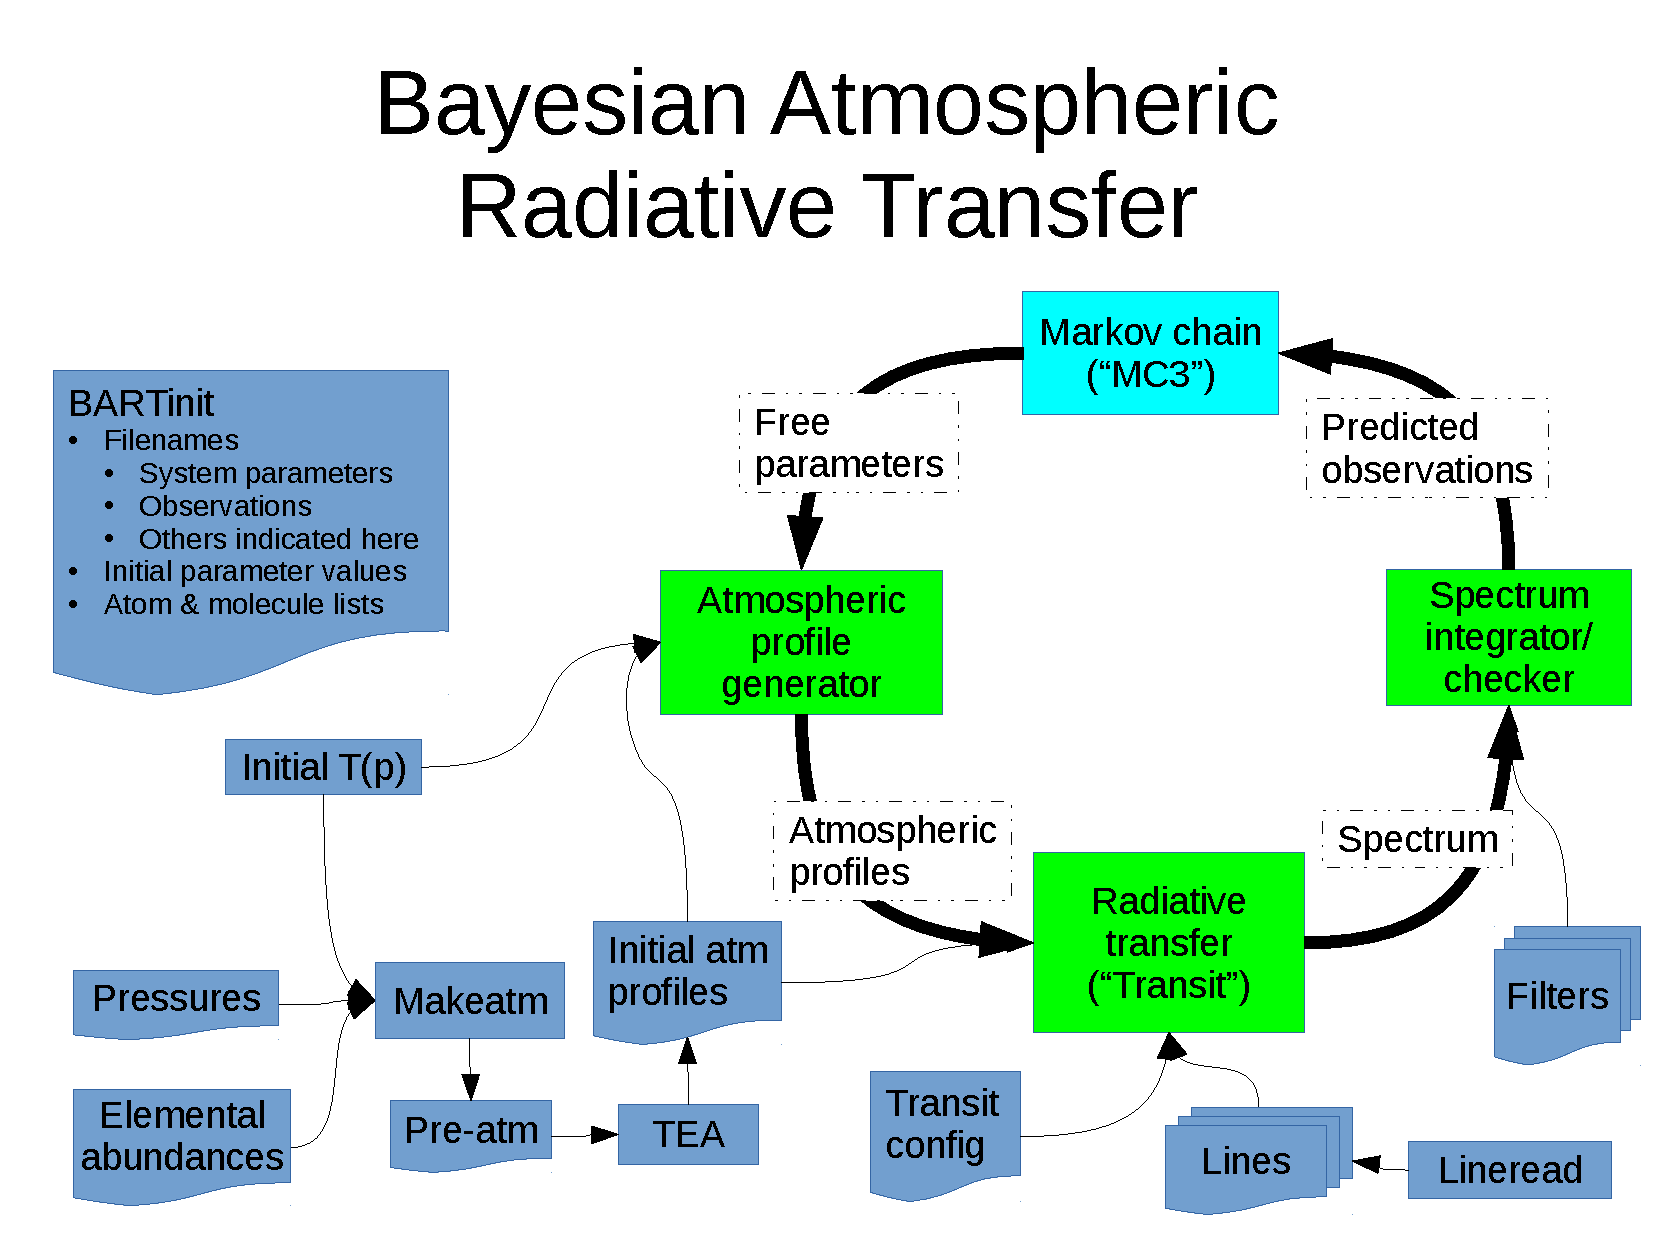
\includegraphics[width=0.9\textwidth, clip]{figs/BARTcharts}}
\caption{\small \label{fig:BARTchart} The BART chart. \findme{explain}. \findme{Remove title}.}
\end{figure}
% SOURCE:  /home/patricio/ast/esp01/bart/transit/develop/plots/widths.py


The BART package is organized as follows: \newline
% The framebox and minipage are necessary because dirtree kills the
% indentation.
\noindent\framebox{\begin{minipage}[t]{0.97\columnwidth}%
\dirtree{%
 .1 BART. 
 .2 code. 
 .2 modules. 
 .3 Transit. 
 .4 RT. 
 .4 pylineread. 
 .3 TEA. 
 .4 prepipe.
 .4 tea. 
 .3 MCcubed. 
 .2 inputs. 
 .2 doc. 
 .2 examples. 
}
\end{minipage}}
\vspace{0.7cm}
% \newline is not working here, therefore I use vspace.
% (because dirtree is such a pain in the ass)


\subsection{License}
\label{sec:license}

Bayesian Atmospheric Radiative Transfer (BART), a code to infer
properties of planetary atmospheres based on observed spectroscopic
information. \\

This project was completed with the support of the NASA Planetary
Atmospheres Program, grant NNX12AI69G, held by Principal Investigator
Joseph Harrington. Principal developers included graduate students
Patricio E. Cubillos and Jasmina Blecic, programmer Madison Stemm, and
undergraduates M. Oliver Bowman and Andrew S. D. Foster.  The included
'transit' radiative transfer code is based on an earlier program of
the same name written by Patricio Rojo (Univ. de Chile, Santiago) when
he was a graduate student at Cornell University under Joseph
Harrington.  Statistical advice came from Thomas J. Loredo and Nate
B. Lust. \newline

Copyright (C) 2015 University of Central Florida.  All rights
reserved. \newline

This is a test version only, and may not be redistributed to any third
party.  Please refer such requests to us.  This program is distributed
in the hope that it will be useful, but WITHOUT ANY WARRANTY; without
even the implied warranty of MERCHANTABILITY or FITNESS FOR A
PARTICULAR PURPOSE. \newline

Our intent is to release this software under an open-source,
reproducible-research license, once the code is mature and the first
research paper describing the code has been accepted for publication
in a peer-reviewed journal.  We are committed to development in the
open, and have posted this code on github.com so that others can test
it and give us feedback.  However, until its first publication and
first stable release, we do not permit others to redistribute the code
in either original or modified form, nor to publish work based in
whole or in part on the output of this code.  By downloading, running,
or modifying this code, you agree to these conditions.  We do
encourage sharing any modifications with us and discussing them
openly. \newline

\noindent We welcome your feedback, but do not guarantee support.
Please send feedback or inquiries to: \newline

\noindent Patricio Cubillos $<$\href{mailto:pcubillos@fulbrightmail.org}
                                    {pcubillos[at]fulbrightmail.org}$>$  \\
\noindent Jasmina Blecic    $<$\href{jasmina@physics.ucf.edu}
                                    {jasmina[at]physics.ucf.edu}$>$   \\
\noindent Joseph Harrington $<$\href{jh@physics.ucf.edu}
                                    {jh[at]physics.ucf.edu}$>$  \\


\noindent or alternatively, \newline

\noindent Joseph Harrington, Patricio Cubillos, and Jasmina Blecic \\
UCF PSB 441            \\
4111 Libra Drive       \\
Orlando, FL 32816-2385 \\
USA                    \\

\noindent
Thank you for using BART! \newline

\section{Installation}
\label{sec:installation}

\subsection{System Requirements}
\label{sec:requirements}

BART was developed on a Unix/Linux machine using Python 2.7.6, Numpy
1.8.2, and mpi4py 1.3.1.

\noindent -- Python 2.7.6+. \\
\noindent -- \href{http://www.numpy.org/}{NumPy} 1.8.2+. \\
\noindent -- \href{http://matplotlib.org/index.html}{matplotlib}. \\
\noindent -- \href{https://github.com/sympy/sympy/releases/tag/sympy/0.7.1.rc1}
                  {SymPy} (version 0.7.1.rc1 to ensure better performance) \\
\noindent -- \href{http://mpi4py.scipy.org/docs/usrman/install.html}
                  {mpi4py} 1.3.1+. \\
\noindent -- An MPI distribution (MPICH preferred). \\
\noindent -- A C \findme{which?} compiler. \\
\noindent -- A Fortran \findme{which?} compiler. \\

\subsection{Install and Compile}
\label{sec:install}

To obtain the latest stable version from the BART
\href{https://github.com/exosports/BART/releases}{releases} page
\herenote{(TBD)}.  Alternatively, clone the repository to your local
machine with the following Linux terminal commands. 
%%
First create a top-level directory to place the code:
\begin{verbatim}
mkdir BART_demo/
cd BART_demo/
topdir=`pwd`
\end{verbatim}
\findme{Backtick marks don't work when copy-pasting text to the terminal.}
\newline

\noindent Clone the repository with all its sub-modules:
\begin{verbatim}
git clone --recursive https://github.com/exosports/BART BART/
\end{verbatim}

\noindent Compile the transit module programs:
\begin{verbatim}
cd $topdir/BART/modules/transit/
make
\end{verbatim}

\noindent Compile the {\tttm MCcubed} routines:
\begin{verbatim}
cd ../MCcubed/src/cfuncs/
make
\end{verbatim}

\noindent To remove the program binaries, execute (in the respective
directories):
\begin{verbatim}
make clean
\end{verbatim}

\noindent Note that there will be warnings. \\
%\findme{Nate says pypy is a great thing to use. Investigate.} \newline

\section{Quick Example}
\label{sec:quick-example}

The following script lets you quickly fit a methane emission spectrum
model to a set of 10 filters between 2 and 4 {\microns}.  These
instructions are meant to be executed from the shell Linux terminal.  To
begin, follow the instructions in the previous Section to install and
compile the code. Now, create a working directory in your top
directory to place the files and execute the programs:

{\fontsize{9.8}{1em}\selectfont 
\begin{verbatim}
cd $topdir
mkdir run/
cd run/
\end{verbatim}}

\noindent Download the methane line-transition database from the HITRAN server:

{\fontsize{9.8}{1em}\selectfont 
\begin{lstlisting}[breaklines]
wget --user=HITRAN --password=getdata -N https://www.cfa.harvard.edu/HITRAN/HITRAN2008/HITRAN2008/By-Molecule/Compressed-files/06_hit08.zip 
unzip 06_hit08.zip
\end{lstlisting}}


\noindent Copy the pylineread configuration file and run pylineread to
make the transition-line-information (TLI) file:

{\fontsize{9.8}{1em}\selectfont
\begin{verbatim}
cp $topdir/BART/examples/demo/pyline_demo.cfg .  
$topdir/BART/modules/transit/pylineread/src/pylineread.py -c pyline_demo.cfg
\end{verbatim}}

\noindent Copy the transit configuration file and run it to make a
table of opacities:

{\fontsize{9.8}{1em}\selectfont
\begin{verbatim}
cp $topdir/BART/examples/demo/transit_demo.cfg .
$topdir/BART/modules/transit/transit/transit -c transit_demo.cfg --justOpacity
\end{verbatim}}

\noindent Copy the BART configuration file and run the MCMC code to sample the
posteriors:

{\fontsize{9.8}{1em}\selectfont
\begin{verbatim}
cp $topdir/BART/examples/demo/BART.cfg .
$topdir/BART/BART.py -c BART.cfg
\end{verbatim}}

\section{Test Cases}
\subsection{WASP-12b}
The following commands will run a test case for BART, based on eclipse depths from Spitzer observations. This test is intended to be used to check that new additions to the BART code have not broken it. Keep in mind that the MCMC algorithm has an element of randomness and thus the output will not be identical every time, but with enough iterations and/or chains, differences should be small. 
\newline

\noindent Navigate to the correct directory:
{\fontsize{9.8}{1em}\selectfont
\begin{verbatim}
cd $topdir/run/
\end{verbatim}}

\noindent Download the line-list .zip file and unzip:
{\fontsize{9.8}{1em}\selectfont
\begin{verbatim}
\findme{command for download}
unzip -j WASP12b_test_line-list.zip
\end{verbatim}}

\noindent Copy the pylineread configuration file and run pylineread to make a transition-line-information (TLI) file:
{\fontsize{9.8}{1em}\selectfont
\begin{verbatim}
cp $topdir/BART/tests/WASP-12b/pyline.cfg .
$topdir/BART/modules/transit/pylineread/src/pylineread.py -c pyline.cfg
\end{verbatim}}

\noindent Copy the Transiting Exoplanet (TEP) file and Stellar Kurucz file from the tests directory:
{\fontsize{9.8}{1em}\selectfont
\begin{verbatim}
cp $topdir/BART/tests/WASP-12b/WASP-12b.tep ../BART/inputs/tep/WASP-12b.tep
cp $topdir/BART/tests/WASP-12b/wasp12b-fp03k2.pck ../BART/inputs/kurucz/wasp12b-fp03k2.pck
\end{verbatim}}


\noindent Copy the BART configuration file and run BART. This will first generate a table of opacities and then run the MCMC code to sample the posteriors:

{\fontsize{9.8}{1em}\selectfont
\begin{verbatim}
cp $topdir/BART/tests/WASP-12b/BART.cfg .
$topdir/BART/BART.py -c BART.cfg
\end{verbatim}}

\noindent The output should be comparable to the following:

\findme{Put stuff here}


\section{Walkthrough}
\label{sec:walk}

Lengthy and wordy, maybe boring too, explanation of what is BART, what
it does, and how it does it.

Talk about the initialization.  Running TEA, then the MCMC, and
finally the best-fitting run.  Talk about what are the inputs, where
to get them?, what are the outputs.

% \newpage
\section{Program Inputs}
\label{sec:inputs}

The executable BART.py is the main BART program to perform most
calculations.  This program can take command-line arguments or a
configuration file (preferred) to set up the calculation details.

Most of the BART inputs can either be given as pre-existing files or
can be produced upon execution.
BART requires the following input files to run:


\subsection{BART Configuration File}
\label{sec:BARTconfig}
The BART configuration file is the main file that sets the arguments for a BART run. The arguments follow the format {\ttb argument = value}, where {\ttb argument} is any of the possible command-line arguments. While all options can be set from the command line, the number of required arguments makes using a configuration file much easier. Note that some of these argument inputs are files that should exist before running BART.

\findme{Speak about the folder structure}.

\subsection{Transit-Line Information (TLI) File}
\label{sec:TLI}
Transit Line-Information (TLI) files are created by the Pylineread routine placed in the BART/modules/transit/
sub-module. They contain information about the emission and absorption lines of molecules found in the exoplanet's atmosphere which ais necessary to calculate opacity. The file contains the following for each line:
\begin{enumerate}
\item[-]molecule isotope
\item[-]central wavenumber
\item[-]oscillator strength
\item[-]lower-state energy
\end{enumerate}

\noindent
To run this module and produce a transit linelist input (TLI) file do the following:
\noindent
Starting from the top directory, navigate to the pylineread module

\begin{verbatim}
cd BART/modules/transit/pylineread
\end{verbatim}

\noindent
Inside the pylineread directory, make a TLI sub-directory and enter it.

\begin{verbatim}
mkdir TLI
cd TLI
\end{verbatim}

\noindent
Copy the pylineread example configuration file.

\begin{verbatim}
cp ../examples/pyline_example.cfg pyline_run01.cfg
\end{verbatim}

\noindent
Read the configuration file header and download the desired databases with the partition functions from the provided links.\\
\\
\noindent
Edit the configuration file with the following information:

\begin{enumerate}
\item[-] Paths to the databases
\item[-] Types of the input databases
\item[-] Desired output TLI filename
\item[-] Desired initial and final wavelength range in microns
\item[-] Verbosity level
\end{enumerate}

\noindent
Run the pylineread module.

\begin{verbatim}
../src/pylineread.py -c pyline\_run01.cfg
\end{verbatim}

\noindent
This will produce the TLI file with the requested name. If unspecified, the file will be placed in the current working directory (/TLI). Otherwise, it will be place in the specified directory. A more in-depth description of the TLI files and the pylineread module can be found in the \href{https://github.com/exosports/transit/blob/master/doc/transit_user_manual.pdf}{Transit User Manual}.


\subsection{Cross-section (CS) File}
\label{sec:CS}
Cross-section (CS) files contain information for any opacity continuum. They must be in HITRAN cross-section format. Several Collision-Induced Absorption (CIA) files are included in the BART/modules/transit/inputs/ directory. These may be used as CS files and are named according to the molecular collisions they represent.

CS files are handled by {\tt Transit} and thus a more in-depth description can be found in the \href{https://github.com/exosports/transit/blob/master/doc/transit_user_manual.pdf}{Transit User Manual}.

\subsection{Transiting Extrasolar Planet (TEP) File}
\label{sec:TEP}
Transiting Extrasolar Planet (TEP) files contain information about the particular exoplanet in question. The file includes many orbital geometry parameters necessary for spectral calculation. Some TEP files can be found in the BART/modules/transit/inputs/tep/ directory.

TEP files are handled by {\tt Transit} and thus a more in-depth description can be found in the \href{https://github.com/exosports/transit/blob/master/doc/transit_user_manual.pdf}{Transit User Manual}.

\subsection{Stellar Spectrum File}
\label{sec:stellarSpec}
The stellar spectrum is provided by a Kurucz stellar spectrum file. They are dependent on the star's metallicity and can be found on \href{http://kurucz.harvard.edu/grids.html}{Robert Kurucz's website}. Some Kurucz files are provided in the BARt/inputs/kurucz directory.

Kurucz stellar spectrum files are handled by {\tt Transit} and thus a more in-depth description can be found in the \href{https://github.com/exosports/transit/blob/master/doc/transit_user_manual.pdf}{Transit User Manual}.

\subsection{Elemental Abundances File}
\label{sec:elemAbund}
The elemental abundances file contains solar abundances of many elements (and some isotopes), along with atomic number, atomic symbol, atomic name, and molar mass. This file is used by TEA to calculate thermochemical equilibrium abundances. The solar abundances as found by Asplund et al, 2009 are found in the BART/inputs/abundances\_Asplund2009.txt file.

\subsection{Filter Files}
\label{sec:filters}
The filter files tell BART how to integrate over the {\tt transit} output spectrum to compare with the given data points. They consist of two columns: wavenumber and filter efficiency. BART will interpolate the spectrum to the filter wavenumbers and multiply the spectrum by the filter before integrating over the bandpass.

Several {\em Spitzer} filter files are provided in the BART/inputs/filters directory.


\subsection{Command-Line Arguments}
\label{sec:configfile}

The user provides the BART configuration arguments in a configuration
file.  The configuration file follows the
\href{https://docs.python.org/2/library/configparser.html}{ConfigParser}
format.   See, e.g., the example below:

\begin{plain}
[MCMC]
# Output directory:
loc_dir = HD209458b

# Elemental species:
in_elem  = H He C N O

# Eclipse-depth data:
data   = 0.00119       ; Spitzer 3.6 microns
         0.00123       ; Spitzer 4.5 microns
\end{plain}

The {\tt[MCMC]} line defines a section (do not edit this line).
Argument entries are input in the format: {\tttb `parameter = value'}.
Multiple valued arguments are set either with blank spaces or in
separated lines.  Blank lines are allowed.  Lines beginning with the
{\tttb `\#'} or the {\tttb `;'} characters are comments and are ignored
by the code.  The {\tttb `;'} character can also be use as an in-line
comment.


\subsubsection{General Arguments}
\label{sec:CLAgen}

\argument{-h, {-}{-}help}{Show the help message and exit.}
\argument{-c FILE, {-}{-}config\_file FILE}{Configuration filename (string).}
\argument{-v INT, {-}{-}verbose-level VERB}{Verbosity level (integer).}
\argument{{-}{-}justTEA}{Run only TEA.}
\argument{{-}{-}justOpacity}{Run just Transit and quit after generating opacity table.}
\argument{{-}{-}resume}{Resume a previous run.}
\argument{{-}{-}tint FLT}{Internal temperature of the planet.}
\argument{{-}{-}filter FILE}{Filter file names (corresponding to data).}
\argument{{-}{-}kurucz\_file FILE}{Kurucz file name.}
\argument{{-}{-}solution STR}{Solution type (transit or eclipse).}

\subsubsection{Atmospheric Pressure Layers}
\label{sec:CLApress}

\argument{{-}{-}n\_layers INT}{Number of atmospheric layers.}
\argument{{-}{-}p\_top DBL}{Pressure at the top of the atmosphere (bars).}
\argument{{-}{-}p\_bottom DBL}{Pressure at the bottom of the atmosphere (bars).}
\argument{{-}{-}log BOOL}{Use log (True) or linear (False) scale sampling.}
\argument{{-}{-}press\_file FILE}{Input/Ouput file with pressure array.}

\subsubsection{Atomic Abundances}
\label{sec:CLAabun}

\argument{{-}{-}abun\_basic FILE}{Input elemental abundances file.}
\argument{{-}{-}abun\_file  FILE}{Inpu/Output modified elemental abundances file.}
\argument{{-}{-}solar\_times INT}{Multiplication factor for metal abundances.}
\argument{{-}{-}COswap BOOL}{Swap Carbon and Oxygen abundances if True.}

\subsubsection{Temperature Profile}
\label{sec:CLAtemp}

\argument{{-}{-}PTtype STR}{Temperature profile model ('line' or 'madhu')}
\argument{{-}{-}PTinit DBL}{1D array of initial temperature profile model parameters.}

\subsubsection{Atmospheric File (TEA) Arguments}
\label{sec:CLAtea}

\argument{{-}{-}in\_elem STR}{1D array of input elements.}
\argument{{-}{-}out\_spec STR}{Output species to include in the atmospheric model}
\argument{{-}{-}preatm\_file FILE}{Pre-atmospheric file name (with elemental abundances per layer.}
\argument{{-}{-}atmfile FILE}{Atmospheric model file (output).}
\argument{{-}{-}uniform DBL}{If not None, 1D array of uniform abundances for each species in out\_spec.}
\argument{{-}{-}refpress FLT}{Reference pressure level (bars) corresponding to the planet radius.}

\subsubsection{MCMC Arguments}
\label{sec:CLAmcmc}

\argument{{-}{-}params DBL}{Initial model-fitting parameters.}
\argument{{-}{-}molfit STR}{1D string array of molecules to fit.}
\argument{{-}{-}Tmin FLT}{Lower temperature boundary (K).}
\argument{{-}{-}Tmax FLT}{Upper temperature boundary (K).}
\argument{{-}{-}quiet}{Set verbosity to minimum.}
\argument{{-}{-}stepsize FLT}{1D array of parameter step sizes.}
\argument{{-}{-}burnin INT}{Number of burn-in iterations per chain.}
\argument{{-}{-}data FLT}{1D array of eclipse/transit depths.}
\argument{{-}{-}uncert FLT}{1D array of data uncertainties.}

\subsubsection{Transit Arguments}
\label{sec:CLAtran}

\argument{{-}{-}tconfig FILE}{Transit configuration file.}
\argument{{-}{-}opacityfile FILE}{Opacity table file (created if nonexistant).}
\argument{{-}{-}outflux FILE}{Ouput file with flux values (for eclipse geometry).}
\argument{{-}{-}outmod FILE}{Output file with modulation values (for transit geometry).}
\argument{{-}{-}shareOpacity BOOL}{If True, use shared memory for the Transit opacity file.}

\subsection{Configuration File}
\label{sec:arguments}


\section{Program Outputs}
\label{sec:outputs}

BART submodules produce the following outputs:

\begin{enumerate}

\item[*]TEA produces one output file:
\begin{enumerate}
\item[-]1. atmopsheric\_file.tea. This file and the BART modified version are placed in the BART output folder
\end{enumerate}

\item[*] MCcubed produces one output file:
\begin{enumerate}
\item[-]1. output.npy - a binary file containing 3D array of parameters per each chain and each iteration
\end{enumerate}

\item[*]{\tt Transit} produces three output files:
\begin{enumerate}
\item[-]1. \_toomuch.dat - list of radii at each wavelength sample where the optical depth reaches the maximum 'toomuch' value

\item[-]2. \_sampling.dat - provides sampling information 

\item[-]3. \_spectrum.dat - gives the flux/modulation (eclipse/transit geometry) vs. wavelength
\end{enumerate}

\item[*] BART produces the following output files:
\begin{enumerate}
\item[-]1. output files:
\begin{enumerate}
\item[-] band\_eclipse.npy - a binary file containing 3D array of eclipse depths per each chain and each iteration
\end{enumerate}
\item[-]2. plots:
\begin{enumerate}
\item[-] best fitting T-P profile with boundaries
\item[-] best fitting abundances
\item[-] contribution functions
\item[-] normalized contribution functions
\item[-] posterior histograms
\item[-] posterior correlation plots
\item[-] spectrum
\end{enumerate}
\end{enumerate}

\end{enumerate}
\section{Running BART}
\label{sec:running}

From the top directory (location of BART), make a current working directory and move into it:

\begin{verbatim}
mkdir run
cd run
\end{verbatim}

\noindent
In the BART/examples/ folder, an example of the BART configuration
file is provided. Copy the BART.cfg example file to the run/ directory:

\begin{verbatim}
cp BART/examples/BART.cfg BART.cfg
\end{verbatim}

\noindent
Edit the file with the correct information:
\begin{enumerate}

\item Give paths to the input tep and kurucz files and the output
     directory

\item ::: Atmospheric pressure layers :::
     Provide the information needed to make a pressure file with desired
     number of layers, range and scale.

\item ::: Elemental-abundances file :::
    Provide the name of the basic abundances files, information how it
    needs to be changed, and the desired name of the final abundances
    file.

\item ::: Temperature profile :::
    There two parametrized temperature-pressure profiles that BART
    can work with: Madhu (based on Madhusudhan adn Seager 2009) and
    Line (based on Line et al 2013). Provide the model type and
    its initial parameter values.

\item ::: Atmospheric Elemental Abundances (pre-atmospheric) File :::
    Provide the name of the desired pre-atmospheric file that will
    contain the temperature-pressure and elemental abundances information
    for each layer in the atmosphere, and desired elemental and molecular
    species. Note: the output species names must use naming convention
    produced by the ../modules/TEA/ module.

\item ::: Atmospheric File (P, T, species-abundances)  :::
     Provide the desired name of the final atmospheric file, that will
     be used as input for ../modules/transit/ module.

\item ::: MCMC arguments  :::
     Provide information to run ../modules/mccubed/ module:
     \begin{enumerate}
    \item[-]eclipse/transit depths and their uncertainties
    \item[-]path to the filter files
    \item[-]3-element tuple to locate the fitting function
         (function\_name routine\_name path\_to\_routine)
    \item[-]list of molecules that have line list data
    \item[-]temperature boundaries (this information depends on the
         line-list and CS databases temperature range)
    \item[-]model fitting parameters (temperature-pressure and abundances
         scale factors).
    \item[-]set basic MCMC variables and define the filename to store
         model fit
    \item[-]set desired verbosity level
     \end{enumerate}

\item ::: Transit variables  :::
     Provide information to run ../modules/transit module:
     \begin{enumerate}
    \item[-]set the desired name of the ../modules/transit/ module
         configuration file that will be produced based on the
         information provided in this section
    \item[-]locate TRANSIT line information and CS files
    \item[-]spectrum information (Note: The range given must be within
         the wavelength range given for the TLI file creation)
    \item[-]the desired geometry solution (transit or eclipse),
         max optical depth, and number of HWHM for Voight profile
         calculation
    \item[-]planetary surface gravity and reference radius and pressure
    \item[-]opacity lines' strength threshold
    \item[-]information to make an opacity-grid file.
        \begin{enumerate}
        \item If variable values and new file name is provided,
            the opacity grid file will be made. This information
            must include the temperatures from the atmospheric file.
            Execution takes couple of hours.
        \item If the opacity file already exists give the path to it.
            Other variables are ignored. Execution will be successful
            only if the pressure and wavenumber samplings are exactly
            the same as in the atmospheric and TLI file, respectively.
            Execution takes around 15 seconds.
        \item If opacityfile name is commented, the opacity calculation
            will be done on spot. Execution takes couple of minutes.
        \end{enumerate}
    \item[-]provide the desired names of the output files
    \end{enumerate}
\end{enumerate}

% + Clone repo
% + Compile code
% + Generate TLI file:
%   - Download database info
%   + Set up pylineread
%   + Run pylineread
% - Generate Opacity file:
%   - Set up Transit 
%   - Run Transit
% - Set up Config files

\subsection{Real-Case Run}

This example shows how to approach a real-life BART run.  In this case you don't want to use demo files (Section \ref{sec:quick-example}), because it uses many defaults that need to be specified for a given analysis.  See below a step-by-step guide to analyze a planet.

\begin{enumerate}

\item  Clone the BART repository to your working directory (See Section \ref{sec:install}).

\item Copy this BART configuration file: BART/examples/BART\_example.cfg  to your run folder.  Start editing the arguments in the configuration file.

\item Determine what observing geometry you will test, and set {\tttb solution} to eclipse or transit accordingly.  Based on that, search for the available data (eclipse or transit depth, respectively) from the literature or your own data analysis.  Put those values in the {\tttb data} and {\tttb uncert} arguments.

\item For each data point, you will need to search for/make the instrumental transmission filter file (See Section \ref{sec:filters}).  Most observatories provide the filter files, but make sure that the file has the right format (Sec. \ref{sec:filters}), edit if needed.  If you use spectroscopic data (e.g., HST's WFC3 data), you will have to reproduce the data analysis of the observer (downsampling, spectral binning).  Set the path to the filter files in the {\tttb filter} argument.

\item Find/make a TEP file for your planet (See Section \ref{sec:TEP}).  In practice, the only parameters that BART requires are the stellar temperture, the stellar radius, the semi-major axis, the planetary radius, the planetary mass, and the stellar $\log(g)$.  This information can be typically found in \href{http://exoplanets.org/}{exoplanets.org/} or \href{http://exoplanet.eu/}{exoplanet.eu/}.  Set the path to the file in {\tttb tep\_name}.

\item Find a Kurucz stellar file (See Section \ref{sec:stellarSpec}).
Follow instructions in /home/esp01/doc/info\_kurucz.
\findme{Copy those instruction here or in Sec \ref{sec:stellarSpec}}
Set the path to the Kurucz file in {\tttb kurucz}.

\item Run pylineread to make a TLI file for the species of interest
(See Section \ref{sec:TLI}).  Set the path to the TLI file in {\tttb linedb}.

\item Determine if you want to load an existing atmospheric file
or create a new one.  If the former, set {\tttb atmfile} to an existing file (and skip to step (\ref{item:molfit})) If you did not change any atmospheric parameters, loading an existing file can save several minutes of runtime.

\item Set the atmospheric pressure layers with the {\tttb press\_file}, 
{\tttb n\_layers},  {\tttb p\_top}, {\tttb p\_bottom}, and {\tttb log}
arguments.

\item Set the initial atmospheric temperature profile.  Set with {\tttm PTtype} if you want to use a model as in \citet{LineEtal2013apjRetrievalI} or  \citet{MadhusudhanSeager2009ApJ-AbundanceMethod}.  Adjust the model parameters in {\tttb PTinit} to set the temperature profile (See Section \ref{sec:PT}).  What is an appropriate initial temperature profile? That is a question yet to be answered.  Having no prior knowledge on the planet's properties, temperatures around the equilibrium temperature would be an initial guess. As a help, run the scripts in \href{https://github.com/exosports/BART/blob/master/scripts/quickguide.py}{BART/scripts/quickguide.py} to see how the temperature profile looks for a given set of model parameters. If TEA is creating a new atmospheric file it will allow you to inspect the profile before continuing.

\item Determine the species present in the atmosphere by setting the
{\tttb out\_spec} argument.  Follow the instruction in Section
\ref{sec:FINDME}.

\item Determine if you want to start with an atmosphere in
thermochemical equilibrium or with uniform species abundances.  
If the former, BART will calculate the abundances with the TEA module.
Determine the elemental abundances by adjusting the {\tttb abun\_basic},
\newline {\tttb solar\_times}, {\tttb COswap}, {\tttb abun\_file},
{\tttb preatm\_file}, and {\tttb in\_elem} arguments (See Section
\ref{sec:FINDME}).

\item If the user chooses to use vertical-uniform abundance profiles.
Set in the {\tttb uniform} argument the desired species abundances
(the order must match that of the {\tttb out\_spec}).

\item \label{item:molfit} Set in {\ttb molfit} the species whose
abundances  you want to fit.

\item Set in {\tttb Tmin} and {\tttb Tmax} the minimum and maximum
boundaries of the temperature profiles to sample.  These boundaries
should not lie beyond the limits set by the TLI and CS data.

\item The {\tttb params} argument sets the initial guess for the list
of fitting parameters. This list corresponds (in this specific order)
the list of the temperature-model parameters (defined by {\tttb PTtype}),
the planetary 'surface' level (only for transit geometry), and the
species abundances (defined by {\tttb molfit}).

\item The {\tttb pmin} and {\tttb pmax} arguments set the fitting parameter-phase space boundaries.

\item The {\tttb stepsize} determines the initial stepsize and which
fitting parameters are free or fixed (See Section \ref{sec:MC3}).

\item See Section \ref{sec:MC3} to lear about the rest of MCMC arguments.

\item wllow and wlhigh set the spectrum boundaries.  What's important
to mention is that we are limited by the boundaries in the CS files.
They go from \sim0.6 um to 400um. Thus, for the moment don’t go shorter
than 0.6um. Also, the shorter the wllow value, the computation time
increases (more than linearly (the spectrum is equi-spaced in wavenumber)),
so stay as close to the shortest filter boundary as possible.

\item For the rest of the wavelength/wavenumber arguments, the defaults
are ok.  Again, ask me if the descriptions are not clear.

\item The tlow, thigh, temp-delt, opacityfile arguments make the opacity file.

\item If you do transit geometry instead of eclipse, you will need to change outflux to outmod.
\end{enumerate}


See the \href{https://github.com/exosports/transit/blob/master/doc/transit_user_manual.pdf}{transit documentation}  to learn more
about all the Transit settings. Keep in mind that it is undergoing constant change, but most of the
info is current.

\subsection{Before Running}
Before running the BART code, we need to generate the required input
files.  A Transit-Line-Information (TLI) file and an Opacity-Grid
file.

\subsubsection{TLI file}

These are quick guidelines to generate a TLI file with the Transit's
pylineread module.  For a detailed description see the \href{https://github.com/exosports/transit/blob/master/doc/transit_user_manual.pdf}{Transit User Manual}. The following lines are intended to be run from the terminal. \\

\noindent
From the BART directory, make a TLI directory and move into it:

\begin{verbatim}
mkdir TLI
cd TLI
\end{verbatim}

\noindent
Copy a pylineread configuration-file template: 
\begin{lstlisting}[breaklines]
cp ../modules/transit/pylineread/examples/pyline_example.cfg ./pyline.cfg
\end{lstlisting}

\noindent
Edit the configuration file and run it: 
\begin{verbatim}
../modules/transit/pylineread/src/pylineread.py -c ./pyline.cfg
\end{verbatim}

\noindent
Runtime can vary from a few minutes to an hour, depending on the number of line databases included. At the end, a TLI file will be saved in the working directory with the specified name.

\subsubsection{Cross-section file}
See the Transit user's manual to set up a Cross-section
file.

\subsubsection{Atmospheric file}
Should I start with the chicken or the egg? \newline
\findme{Something like (to run just the atmosphere part):} \\
{\tttb ../BART.py --atmosphere}  \\

\findme{jh is not happy with the file extensions.}

\subsubsection{Opacity file}

\findme{If BART doesn't find these files, the code should created them
  before running.} \\

These are quick guidelines to generate an Opacity-grid file with
Transit.  For a detailed description see the Transit user's manual. \\

Create a directory to run Transit and place the Opacity file: \newline
{\tttb cd ../}        \\
{\tttb mkdir Opacity} \\
{\tttb cd Opacity}    \\

Copy a Transit configuration-file template: \newline
{\tttb cp ../modules/transit/run/config\_sample.cfg ./opacity.cfg}  \\

Edit the configuration file and run it: \newline
{\tttb ../modules/transit/transit/transit -c opacity.cfg}  \\

\findme{It would be nice to run Transit from BART, something like:} \\
{\tttb ../BART.py --opacity}  \\

% {\tttb }  \\

\subsubsection{TEA setup}

Copy the BART and TEA configuration-file templates from the examples
directory into your running dir, e.g.: \newline
{\tttb cp ../myBART/examples/BART.cfg .}  \\
{\tttb cp ../myBART/examples/TEA.cfg .}   \\

Edit the parameters in the TEA configuration file. \findme{Set this up
  from the BART config file}
\begin{plain}
# === Full path to TEA package ===
location_TEA = ../modules/TEA/

# === Full path to abundances file ===
abun_file = ../modules/TEA/lib/abundances.txt

# === Full path to TEA working directory ===
location_out = ./HD209458b/
\end{plain}

Even though transit has many command-line arguments, only a few of
them are strictly necessary for a run.  See for example the file in
{\tttm mytransit/examples/example03.cfg}.  \findme{For Jasmina: see
  \newline
  /home/patricio/ast/esp01/bart/transit/develop/examples/example03.cfg}

\subsubsection{BART setup}

BART can be run from any folder, provided the user gives the path to
the executable.  We recommend to create a folder exclusively dedicated
to run and hold the transit results to keep the results organized,
e.g.: \\
{\tttb cd myBART/}   \\
{\tttb mkdir run}    \\
{\tttb cd run/}      \\

The BART code consists of an initialization step and the proper MCMC
run on the spectrum modeling.

% \section{Code Organization}
% \label{sec:organization}

% \findme{TBD}

% \section{Routines}
% \label{sec:routines}

% \findme{TBD}

\section{Be Kind}
\label{sec:bekind}
Please cite these papers if you found this package useful for your
research:
\begin{itemize}
\item \href{https://github.com/pcubillos/transit}{Cubillos et
    al. (2015)} (in preparation).

\item \href{https://github.com/dzesmin/}{Blecic et al. (2015)} (in
            preparation).
\item \href{https://github.com/dzesmin/}{Harrington et al. (2015)} (in
            preparation).
\end{itemize}
Thanks!

% \section{Further Reading}
% \label{sec:furtherreading}

% TBD: Add papers here.

\bibliography{BART_user_manual}
%\nobibliography{BART_user_manual}

\end{document}
